% Rešerše – iDoklad (vkládá se do kapitoly 01-reserse.tex)
\section{iDoklad}\label{sec:reserse-idoklad}

iDoklad je online fakturační a~evidenční služba ze skupiny, do které patří i~ekonomické systémy Money. Základní údaje shrnuje tabulka~\ref{tab:reserse-idoklad}.

\begin{table}[H]
\centering
\small
\begin{tabular}{>{\raggedright\arraybackslash}p{0.24\linewidth}>{\raggedright\arraybackslash}p{0.70\linewidth}}
\hline
\textbf{Kritérium} & \textbf{Zjištění} \\
\hline
Název & iDoklad \\
Společnost & Seyfor, a.s. (CZ; dříve Solitea) \cite{idoklad-web} \\
Typ aplikace & webová aplikace a~mobilní aplikace pro iOS a~Android \cite{idoklad-web,idoklad-vlastnosti} \\
Hostování & pouze cloud (SaaS provozovaný výrobcem); vlastní server ani lokální instalace nejsou možné \\
Licence & proprietární, předplatné \\
Cena & ceny bez DPH za měsíc při roční / čtvrtletní / měsíční platbě: Zdarma 0~Kč (1 uživatel, 5 kontaktů), Základní 187 / 220 / 240~Kč (2 uživatelé), Oblíbený 358 / 397 / 430~Kč (5 uživatelů), Prémiový 625 / 703 / 750~Kč (9 uživatelů) \cite{idoklad-cenik} \\
Zkušební verze & 60 dní v~tarifu Prémiový, bez platební karty; garance vrácení peněz do 30 dní \cite{idoklad-cenik,idoklad-vlastnosti} \\
\hline
\end{tabular}
\caption{Základní údaje o~řešení iDoklad}\label{tab:reserse-idoklad}
\end{table}

\subsection{Zkušenosti ze zkušební verze}

První dojem z~aplikace je velmi příjemný. Navigace je umístěna v~levém panelu s~ikonami, který lze zasunout a~získat tak více místa, což odpovídá návrhu navrhované aplikace. Výrazné zelené tlačítko \emph{Nový} umožňuje vytvořit libovolný doklad bez hledání v~záložkách. Tabulky faktur, nabídek i~ceníku vypadají jednotně, zobrazují jen potřebné sloupce a~další lze doplnit v~nastavení. Formulář cenové nabídky je totožný s~formulářem faktury, což usnadňuje orientaci. Sloupec se stavem dokladu přehledně ukazuje, v~jaké fázi se dokument nachází.

Formulář faktury zobrazuje poměrně mnoho údajů najednou, všechny však mají svůj smysl. Chybějící údaje jsou na rozdíl od Fakturoidu zobrazeny pouze jako varování ve spodní části formuláře a~doklad lze tlačítkem \emph{Přesto uložit} uložit i~s~nimi (obrázek~\ref{obr:idoklad-faktura}). Pořadové číslo dokladu lze změnit, formát číselné řady se ale nastavuje zástupnými znaky podobně jako ve Fakturoidu, i~když nápověda jejich význam vysvětluje. Tisk zobrazí náhled dokumentu, vzhled je však možné volit jen z~předdefinovaných variant a~funkce \emph{Šablony} slouží, stejně jako ve Fakturoidu, pouze k~předvyplnění opakovaných dokladů. Ceníkové položky stačí zadat jen názvem, ostatní údaje nejsou povinné. Velmi zdařilá jsou drobná vyskakovací oznámení, která jsou výrazná, ale nepřekážejí a~rychle zmizí, a~panel upozornění, který by v~navrhované aplikaci mohl sloužit pro upomínky blížících se termínů nebo historii posledních změn.

\begin{figure}[H]
\centering
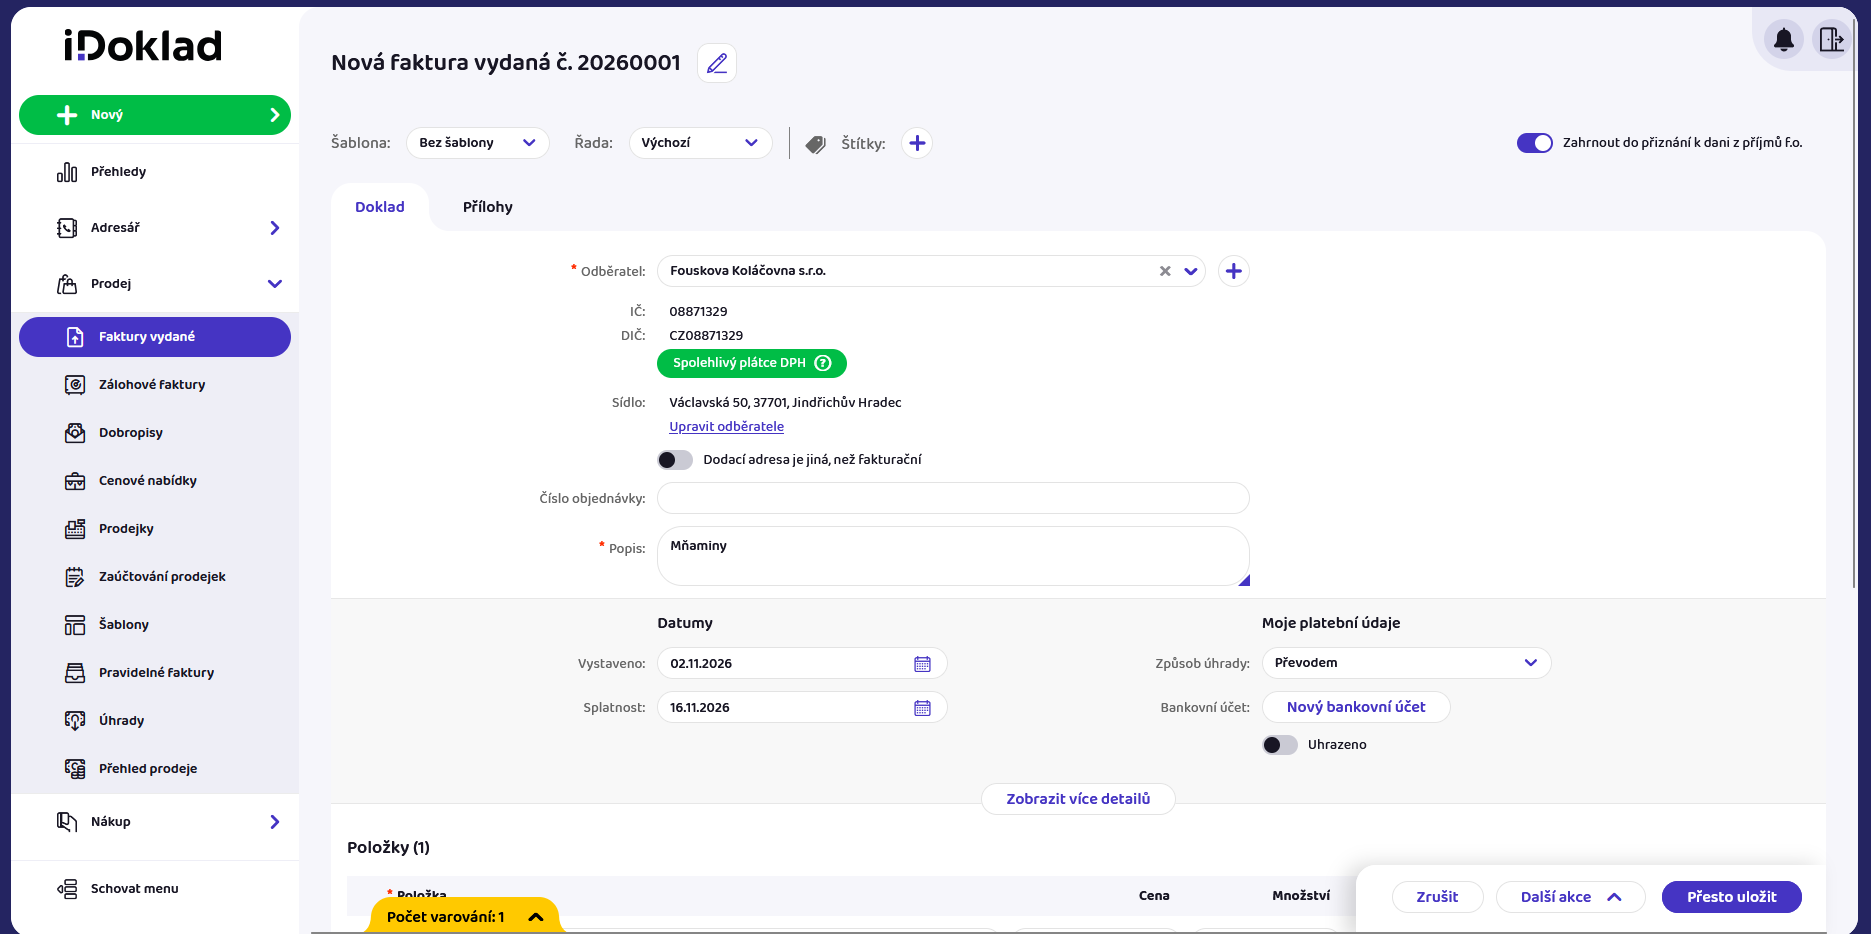
\includegraphics[width=\linewidth]{obrazky/reserse/iDoklad_tvorba_faktury.png}
\caption{Formulář nové faktury v~aplikaci iDoklad s~varováním o~chybějících údajích a~tlačítkem \emph{Přesto uložit} (zdroj: vlastní snímek obrazovky ze zkušební verze, pořízeno 2.~11.~2026)}\label{obr:idoklad-faktura}
\end{figure}

Nevýhodou je velké množství ikon s~akcemi přímo v~seznamu dokladů, z~nichž řada není pro běžnou práci potřeba a~stačila by v~detailu dokladu. Filtrování podle stavu (\emph{Všechny}, \emph{Uhrazené} atd.) je řešeno samostatnými položkami v~menu, přitom by stačil štítek se stavem u~každého dokladu a~filtr v~tabulce. Některé stránky nemají tlačítko \enquote{Zpět} a~ikona v~pravém horním rohu, která by jej mohla nahrazovat, uživatele odhlásí. Právě proto se navrhovaná aplikace drží doporučené zásady konzistence: tlačítka se stejným účelem mají na všech obrazovkách stejné umístění i~vzhled (oddíl~\ref{sec:ui-soulad}). Stejné nastavení seznamu je dostupné ze dvou různých tlačítek a~ve spodní části obrazovky se opakovaně zobrazuje propagace aplikace. Sekce Nákup (přijaté faktury, účtenky, Inbox) a~řada dokladů v~sekci Prodej (zálohové faktury, dobropisy, prodejky, pravidelné faktury) přesahují potřeby malé servisní firmy. Zajímavou inspirací pro možné rozšíření je naopak sekce Finance s~pokladnou pro evidenci hotovostních plateb.

Stejně jako Fakturoid je iDoklad primárně fakturační aplikace a~chybí v~něm evidence zakázek, zařízení, provedené práce a~kalendář.

\subsection{Vhodnost pro malé firmy}

iDoklad je vhodný pro živnostníky a~malé obchodní firmy, zejména pokud spolupracují s~externí účetní, která používá systémy Money nebo Pohoda \cite{idoklad-ucetni}. Jednotné a~přehledné rozhraní a~dlouhá zkušební doba usnadňují začátek. Pro servisní firmu ale pokryje opět jen fakturaci, data jsou uložena výhradně v~cloudu výrobce a~vyšší tarify jsou dražší než u~Fakturoidu.
